%%%%%%%%%%% Aquí va la solución al problema 3.
\newpage
\textbf{\textcolor{MidnightBlue}{3.}}
¿El árbol generador de la figura 1 puede obtenerse en alguna ejecución del algoritmo
BFS visto en clase? de ser el caso, describe la ejecución, y de no serlo, explica por qué no se puede.
Haz lo mismo con el algoritmo DFS.\\

\begin{center}
        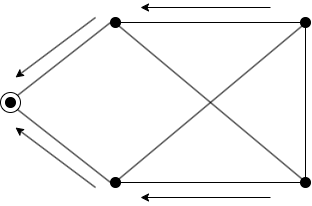
\includegraphics[scale=0.7]{grapho.png}
    \end{center}
Para poder visualizar mejor el árbol se le asigno un identificador a cada uno de
sus nodos ($A,B,C,D,E$)\\

A) Caso BFS:
    \begin{center}
        \includegraphics[scale=0.8]{grapho1.png}
    \end{center}
Si, bueno como se comienza desde nuestro caso $A$, entonces se declara como padre y este
le manda $<BFS,A>$ tanto a $B$, como $C$, de ahi tanto $B$ y $C$ manda $<BFS,ID>$ a todos sus vecinos,
y al mismo tiempo manda a $A$, definiendolo como su padre. Y asi hasta llegar a nuestro
vértice $D$ el cuál le manda a nuestro vértice $E$. Ya que todos los vértices hayan
recibido su respectivo mensaje con $<BFS,ID>$, devolverán un mensaje a su "padre" por decirlo
así con $<alredy>$. De los vértices que reciban ya sea $<alredy>$ o $<parent>$ se tendrán que cumplir
con la codición dada el algoritmo BFS.\\

B) Caso DFS:\\
    \begin{center}
        \includegraphics[scale=0.8]{grapho2.png}
    \end{center}

Al comenzar desde $A$, se puede obesrvar que solo manda un
mensaje a uno sus posibles vecinos. Por lo que, en cierta forma
obliga a decidir entre varios posibles caminos para distribuir
el mensaje, pero no se puede lograr, generar tal árbol, que se
nos pide, ya que al ser una gráfica con vértices impares, debe haber
habido otro vértice, se pudo haber enviado un mensaje más y así lograr
el árbol objetivo.
